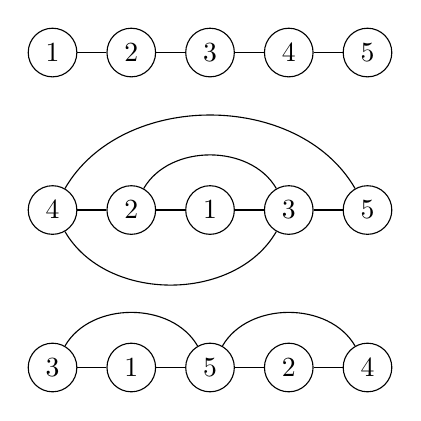
\begin{tikzpicture}[node distance={15mm}, main/.style = {draw, circle}]

    \node[main] (x1) at (0, 4) {$1$};
    \node[main] (x2) at (1, 4) {$2$};
    \node[main] (x3) at (2, 4) {$3$};
    \node[main] (x4) at (3, 4) {$4$};
    \node[main] (x5) at (4, 4) {$5$};
    \draw (x1) -- (x2);
    \draw (x2) -- (x3);
    \draw (x3) -- (x4);
    \draw (x4) -- (x5);

    %--------------------------------------------

    \node[main] (x11) at (0, 2) {$4$};
    \node[main] (x21) at (1, 2) {$2$};
    \node[main] (x31) at (2, 2) {$1$};
    \node[main] (x41) at (3, 2) {$3$};
    \node[main] (x51) at (4, 2) {$5$};
    
    \draw (x11) -- (x21);
    \draw (x21) -- (x31);
    \draw (x31) -- (x41);
    \draw (x41) -- (x51);
    \draw[out=60, in=120] (x21) to (x41);
    \draw[out=-60, in=-120] (x11) to (x41);
    \draw[out=60, in=120] (x11) to (x51);

    %--------------------------------------------

    \node[main] (x11) at (0, 0) {$3$};
    \node[main] (x21) at (1, 0) {$1$};
    \node[main] (x31) at (2, 0) {$5$};
    \node[main] (x41) at (3, 0) {$2$};
    \node[main] (x51) at (4, 0) {$4$};
    
    \draw (x11) -- (x21);
    \draw (x21) -- (x31);
    \draw (x31) -- (x41);
    \draw (x41) -- (x51);
    \draw[out=60, in=120] (x11) to (x31);
    \draw[out=60, in=120] (x31) to (x51);

    
\end{tikzpicture} \\
\begin{tikzpicture}[node distance={15mm}, main/.style = {draw, circle}]



    
\end{tikzpicture} 
    